\documentclass[tikz,border=10pt]{standalone}
\usepackage{tikz}
% \usetikzlibrary{arrows,intersections}

\usepackage{pgfplots}
\pgfplotsset{compat=newest}
\begin{document}
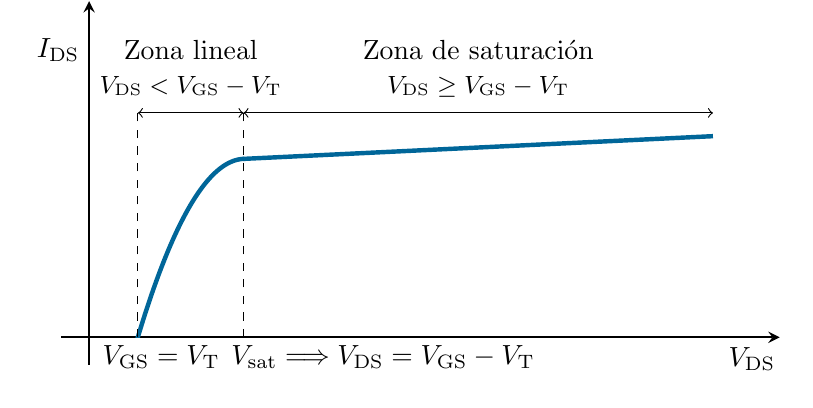
\begin{tikzpicture}[
  circ/.style={
      draw,
      fill = white,ur
      circle,
      inner sep = 0pt,
      minimum size = 4pt,
      every text node part/.style={align=center}
    }]
%  \coordinate (O) at (0,0);
%  \draw[->] (-0.3,0) -- (8.7,0) coordinate[label = {below:$t$}] (xmax);
%  \draw[->] (0,-0.3) -- (0,5) coordinate[label = {right:$f$}] (ymax);
%  \path[name path=x] (0.3,0.5) -- (6.7,4.7);
%  \path[name path=y] plot[smooth] coordinates {(-0.3,2) (2,1.5) (4,2.8) (6,5)};
%  \foreach \ini [evaluate=\ini as \inieval using 2.5*\ini] in {0,...,2}
%\draw[thick,cyan] (\inieval+0.2,1) -- ++(2.5,3) -| (\inieval+2.7,1);
%\draw[thick,cyan] (7.5+0.2,1) -- ++(0.75,0.9);
%
%  \foreach \ini [evaluate=\ini as \inieval using 2.5*\ini] in {0,...,2}
%\draw[ultra thick,color={rgb:red,0;green,1;blue,1.5}] (\inieval+0.7,1) -- ++(2.5,3) -- ++(0,-3.0155);
%\draw[ultra thick,color={rgb:red,0;green,1;blue,1.5}] (8+0.2,1) -- ++(0.25,0.3);
%\draw[ultra thick,color={rgb:red,0;green,1;blue,1.5}] (0.7,1) -- ++(0,3)--++(-0.5,-0.6);
\begin{axis}[
axis y line=center,
axis x line=center,
axis line style = thick,
   domain=0:2,
    samples=4*360,
    xtick=\empty,
    ytick=\empty,
    width=10cm, height=5.5cm,
    xlabel={$V_{\mathrm{DS}}$},
    ylabel={$I_{\mathrm{DS}}$},
    xlabel style={below},
    ylabel style={below left},
    ymin=0,
    xmin=0,
    xmax = 8.5,
    ymax = 1.1,
    axis line style={shorten >=-10pt, shorten <=-10pt}
]
\addplot [ultra thick,color={rgb:red,0;green,1;blue,1.5},domain=0:1.99] {3.363636*(10^(-1))*(2*(x-1-(x-1)^2/2))+0.3};
\addplot [ultra thick,color={rgb:red,0;green,1;blue,1.5},domain=1.98:8] {0.013454544*x+0.6095};
%\addplot [ultra thick,color={rgb:orange,1;yellow,2;pink,5}] {1-3*mod(-x-1.3,5)};
%\addplot [only marks, circ] table {
%6   7.9
%7.1 7.9
%13.1 10.9
%13.1 14.2
%};
\draw[black, <->] (0.625,0.8)--(1.98,0.8) node[midway, above] {\begin{tabular}{c} Zona lineal \\ \small{$V_{\mathrm{DS}} < V_{\mathrm{GS}}-V_{\mathrm{T}}$}\end{tabular}};
\draw[black, dashed] (0.625,0) -- (0.625,0.8) {};
\draw[black, dashed] (1.98,0) -- (1.98,0.8) node[above]{};
%\draw[black, dashed] (1.98,10.9) -- (11.2,10.9) {};
%\draw[black, dashed] (13.1,14.2) -- (11.2,14.2) {};
\draw[black, <->] (1.98,0.8)--(8,0.8) node[midway, above] {\begin{tabular}{c} Zona de saturación \\ \small{$V_{\mathrm{DS}} \geq V_{\mathrm{GS}}-V_{\mathrm{T}}$}\end{tabular}};
\node [above] (n3) at (1.7,-0.03) {};
\node [above] (n5) at (0.924539354138895,-0.03) {};
\end{axis}
\node [below right] (n4) at (n3) {$V_{\mathrm{sat}}\Longrightarrow V_{\mathrm{DS}} = V_{\mathrm{GS}}-V_{\mathrm{T}}$};
\node [below] (n6) at (n5) {$V_{\mathrm{GS}} = V_\mathrm{T}$};
%\draw[blue, <->] (i-2) -- node[right] {$f(x_0 + \varepsilon) - f(x_0)$}
%                              (i-12);
%    \draw[blue, <->] (i-1) -- node[below] {$\varepsilon$} (i-12);
\end{tikzpicture}
\end{document}%


%%\documentclass[14pt]{extarticle}
%%\usepackage{pgfplots}
%%\pgfplotsset{compat=newest}
%%\begin{document}
%%
%%\begin{center}
%%\begin{tikzpicture}%[scale=1.5]
%%\begin{axis}[
%%  samples at={0,0.1,...,10}, % gives a data point every pi/4
%%  xlabel = $t$,
%%  ylabel = $f$,
%%  axis lines = center,
%%  enlargelimits,
%%  every axis x label/.append style = {below},
%%  every axis y label/.append style = {left},
%%  xtick = {-1, 1, 3},
%%  %xticklabels = {$-1$, $1$, $3$}, % not needed, numbers are set in math mode by default
%%\end{axis}
%%\end{tikzpicture}
%%\end{center}
%%
%%\end{document}
%%
%
%
%\documentclass[tikz,border=10pt]{standalone}
%\usetikzlibrary{arrows,intersections}
%\usepackage{tikz}
%\usepackage{pgfplots}
%\pgfplotsset{compat=newest}
%\begin{document}
%	\begin{tikzpicture}[
%	circ/.style={
%		draw,
%		fill = white,
%		circle,
%		inner sep = 0pt,
%		minimum size = 4pt,
%		every text node part/.style={align=center}
%	}]
%	%  \coordinate (O) at (0,0);
%	%  \draw[->] (-0.3,0) -- (8.7,0) coordinate[label = {below:$t$}] (xmax);
%	%  \draw[->] (0,-0.3) -- (0,5) coordinate[label = {right:$f$}] (ymax);
%	%  \path[name path=x] (0.3,0.5) -- (6.7,4.7);
%	%  \path[name path=y] plot[smooth] coordinates {(-0.3,2) (2,1.5) (4,2.8) (6,5)};
%	%  \foreach \ini [evaluate=\ini as \inieval using 2.5*\ini] in {0,...,2}
%	%\draw[thick,cyan] (\inieval+0.2,1) -- ++(2.5,3) -| (\inieval+2.7,1);
%	%\draw[thick,cyan] (7.5+0.2,1) -- ++(0.75,0.9);
%	%
%	%  \foreach \ini [evaluate=\ini as \inieval using 2.5*\ini] in {0,...,2}
%	%\draw[ultra thick,color={rgb:red,0;green,1;blue,1.5}] (\inieval+0.7,1) -- ++(2.5,3) -- ++(0,-3.0155);
%	%\draw[ultra thick,color={rgb:red,0;green,1;blue,1.5}] (8+0.2,1) -- ++(0.25,0.3);
%	%\draw[ultra thick,color={rgb:red,0;green,1;blue,1.5}] (0.7,1) -- ++(0,3)--++(-0.5,-0.6);
%	\begin{axis}[
%	axis y line=center,
%	axis x line=center,
%	axis line style = thick,
%	domain=0:2,
%	samples=4*360,
%	xtick=\empty,
%	ytick=\empty,
%	width=10cm, height=5.5cm,
%	xlabel={$V_{\mathrm{DS}}$},
%	ylabel={$I_{\mathrm{DS}}$},
%	xlabel style={below},
%	ylabel style={below left},
%	ymin=0,
%	xmin=0,
%	xmax = 8.5,
%	ymax = 1.1,
%	axis line style={shorten >=-10pt, shorten <=-10pt}
%	]
%	\addplot [ultra thick,color={rgb:red,0;green,1;blue,1.5},domain=0:1.99] {3.363636*(10^(-1))*(2*(x-1-(x-1)^2/2))+0.3};
%	\addplot [ultra thick,color={rgb:red,0;green,1;blue,1.5},domain=1.98:8] {0.013454544*x+0.6095};
%	%\addplot [ultra thick,color={rgb:orange,1;yellow,2;pink,5}] {1-3*mod(-x-1.3,5)};
%	%\addplot [only marks, circ] table {
%	%6   7.9
%	%7.1 7.9
%	%13.1 10.9
%	%13.1 14.2
%	%};
%	\draw[black, <->] (0.625,0.8)--(1.98,0.8) node[midway, above] {\begin{tabular}{c} Zona lineal \\ \small{$V_{\mathrm{DS}} < V_{\mathrm{GS}}-V_{\mathrm{T}}$}\end{tabular}};
%	\draw[black, dashed] (0.625,0) -- (0.625,0.8) {};
%	\draw[black, dashed] (1.98,0) -- (1.98,0.8) node[above]{};
%	%\draw[black, dashed] (1.98,10.9) -- (11.2,10.9) {};
%	%\draw[black, dashed] (13.1,14.2) -- (11.2,14.2) {};
%	\draw[black, <->] (1.98,0.8)--(8,0.8) node[midway, above] {\begin{tabular}{c} Zona de saturación \\ \small{$V_{\mathrm{DS}} > V_{\mathrm{GS}}-V_{\mathrm{T}}$}\end{tabular}};
%	\node [above] (n3) at (1.7,-0.03) {};
%	\end{axis}
%	\node [below right] (n4) at (n3) {$V_{\mathrm{sat}}\Longrightarrow V_{\mathrm{DS}} = V_{\mathrm{GS}}-V_{\mathrm{T}}$};
%	%\draw[blue, <->] (i-2) -- node[right] {$f(x_0 + \varepsilon) - f(x_0)$}
%	%                              (i-12);
%	%    \draw[blue, <->] (i-1) -- node[below] {$\varepsilon$} (i-12);
%	\end{tikzpicture}
%\end{document}%
